\documentclass[11pt]{article}
\usepackage[margin=1in]{geometry}
\usepackage{amsmath}
\usepackage{graphicx}
\usepackage{listings}
\usepackage{xcolor}
\usepackage{hyperref}

\lstset{
    basicstyle=\ttfamily\small,
    breaklines=true,
    numbers=left,
    numberstyle=\tiny,
    frame=single,
    language=Python,
    showstringspaces=false,
    commentstyle=\color{gray},
    keywordstyle=\color{blue},
    stringstyle=\color{orange}
}

\title{\textbf{SSIE-500: Homework 6} \\ Measuring Complexity of Languages (2)}
\author{Zeinab Davoudmanesh}
\date{November 2025}

\begin{document}

\maketitle

\section{Introduction}
This report presents an analysis of linguistic complexity across three human languages (English, German, and French) using information theory concepts. Specifically, we implement Shannon entropy calculations and Huffman coding to measure and compare the information content and compressibility of real-world texts from classic literature.

\subsection{Objectives}
The assignment consists of five main tasks:
\begin{enumerate}
    \item Calculate the information entropy of character frequency distributions in English text
    \item Implement a Huffman coding algorithm to generate optimal binary codes
    \item Compare average code word length with theoretical entropy
    \item Analyze sentence-level encoding metrics
    \item Repeat the analysis for German and French, and compare results across languages
\end{enumerate}

\subsection{Data Sources}
We use authentic literary texts from Project Gutenberg:
\begin{itemize}
    \item \textbf{English:} Pride and Prejudice by Jane Austen
    \item \textbf{German:} Die Verwandlung (Metamorphosis) by Franz Kafka
    \item \textbf{French:} Les Trois Mousquetaires by Alexandre Dumas
\end{itemize}
For computational efficiency, we analyze the first 100,000 characters from each text after removing Project Gutenberg headers and footers.

\section{Methodology}

\subsection{Information Entropy}
Shannon entropy measures the average information content per character in a text. For a discrete random variable with character set $X$ and probability distribution $p(x)$, entropy $H(X)$ is defined as:
\begin{equation}
    H(X) = -\sum_{x \in X} p(x) \log_2 p(x)
\end{equation}
Higher entropy indicates greater unpredictability and complexity in character usage.

\subsection{Huffman Coding}
Huffman coding is a lossless data compression algorithm that assigns variable-length binary codes to characters based on their frequencies. More frequent characters receive shorter codes, achieving near-optimal compression.

The algorithm works as follows:
\begin{enumerate}
    \item Create a leaf node for each character with its frequency
    \item Build a min-heap from all nodes
    \item Repeatedly extract two nodes with minimum frequency
    \item Create a new internal node with these two nodes as children
    \item Insert the new node back into the heap
    \item Continue until only one node remains (the root)
    \item Assign binary codes by traversing the tree (0 for left, 1 for right)
\end{enumerate}

The average code length $L$ is calculated as:
\begin{equation}
    L = \sum_{x \in X} p(x) \cdot \text{length}(\text{code}(x))
\end{equation}

For optimal prefix-free codes, Huffman coding guarantees: $H(X) \leq L < H(X) + 1$

\section{Results}

\subsection{Character-Level Analysis}
Table \ref{tab:char_level} presents the comparative analysis across all three languages.

\begin{table}[h]
\centering
\begin{tabular}{lcccc}
\hline
\textbf{Language} & \textbf{Entropy} & \textbf{Avg Code Length} & \textbf{Difference} & \textbf{Unique Chars} \\
                  & (bits/char)      & (bits/char)              & (bits)              &                       \\
\hline
English           & 4.5031           & 4.5441                   & 0.0410              & 90                    \\
German            & 4.3903           & 4.4249                   & 0.0346              & 78                    \\
French            & 4.6828           & 4.7130                   & 0.0301              & 102                   \\
\hline
\end{tabular}
\caption{Character-level entropy and Huffman coding results}
\label{tab:char_level}
\end{table}

\textbf{Key Observations:}
\begin{itemize}
    \item French exhibits the highest character-level entropy (4.6828 bits/char), indicating the most diverse character usage among the three languages
    \item German shows the lowest entropy (4.3903 bits/char), suggesting more predictable character patterns
    \item All three languages achieve Huffman coding efficiency exceeding 99\%, with differences between entropy and code length less than 0.05 bits
    \item French has the most unique characters (102), likely due to accented characters
\end{itemize}

\subsection{Sample Huffman Codes}
Table \ref{tab:huffman} shows the top 10 most frequent characters and their assigned Huffman codes for English.

\begin{table}[h]
\centering
\begin{tabular}{ccc}
\hline
\textbf{Character} & \textbf{Huffman Code} & \textbf{Frequency} \\
\hline
(space)            & 00                    & 20075              \\
e                  & 1110                  & 8957               \\
t                  & 1010                  & 6179               \\
a                  & 0111                  & 5458               \\
o                  & 0110                  & 5148               \\
n                  & 0101                  & 5086               \\
i                  & 0100                  & 4877               \\
s                  & 11110                 & 4523               \\
h                  & 11011                 & 4293               \\
r                  & 11001                 & 4182               \\
\hline
\end{tabular}
\caption{Top 10 Huffman codes for English text}
\label{tab:huffman}
\end{table}

Note that the space character, being most frequent, receives the shortest code (2 bits), while less common characters receive longer codes.

\subsection{Sentence-Level Analysis}
Table \ref{tab:sentence} presents the sentence-level encoding results.

\begin{table}[h]
\centering
\begin{tabular}{lccc}
\hline
\textbf{Language} & \textbf{Total Sentences} & \textbf{Avg Bits/Sentence} & \textbf{Std Deviation} \\
\hline
English           & 950                      & 464.03                     & 396.44                 \\
German            & 646                      & 671.82                     & 491.38                 \\
French            & 851                      & 535.81                     & 769.40                 \\
\hline
\end{tabular}
\caption{Sentence-level encoding metrics}
\label{tab:sentence}
\end{table}

\textbf{Key Findings:}
\begin{itemize}
    \item German sentences require significantly more bits on average (671.82 bits), approximately 1.5 times more than English
    \item This reflects Kafka's complex and philosophical sentence structures in \textit{Die Verwandlung}
    \item French shows the highest variability (std = 769.40), indicating a wide range of sentence lengths
    \item English has the most consistent sentence lengths with the lowest standard deviation
\end{itemize}

\subsection{Visualization}
Figure \ref{fig:comparison} presents a comprehensive six-panel visualization comparing all three languages.

\begin{figure}[h]
\centering
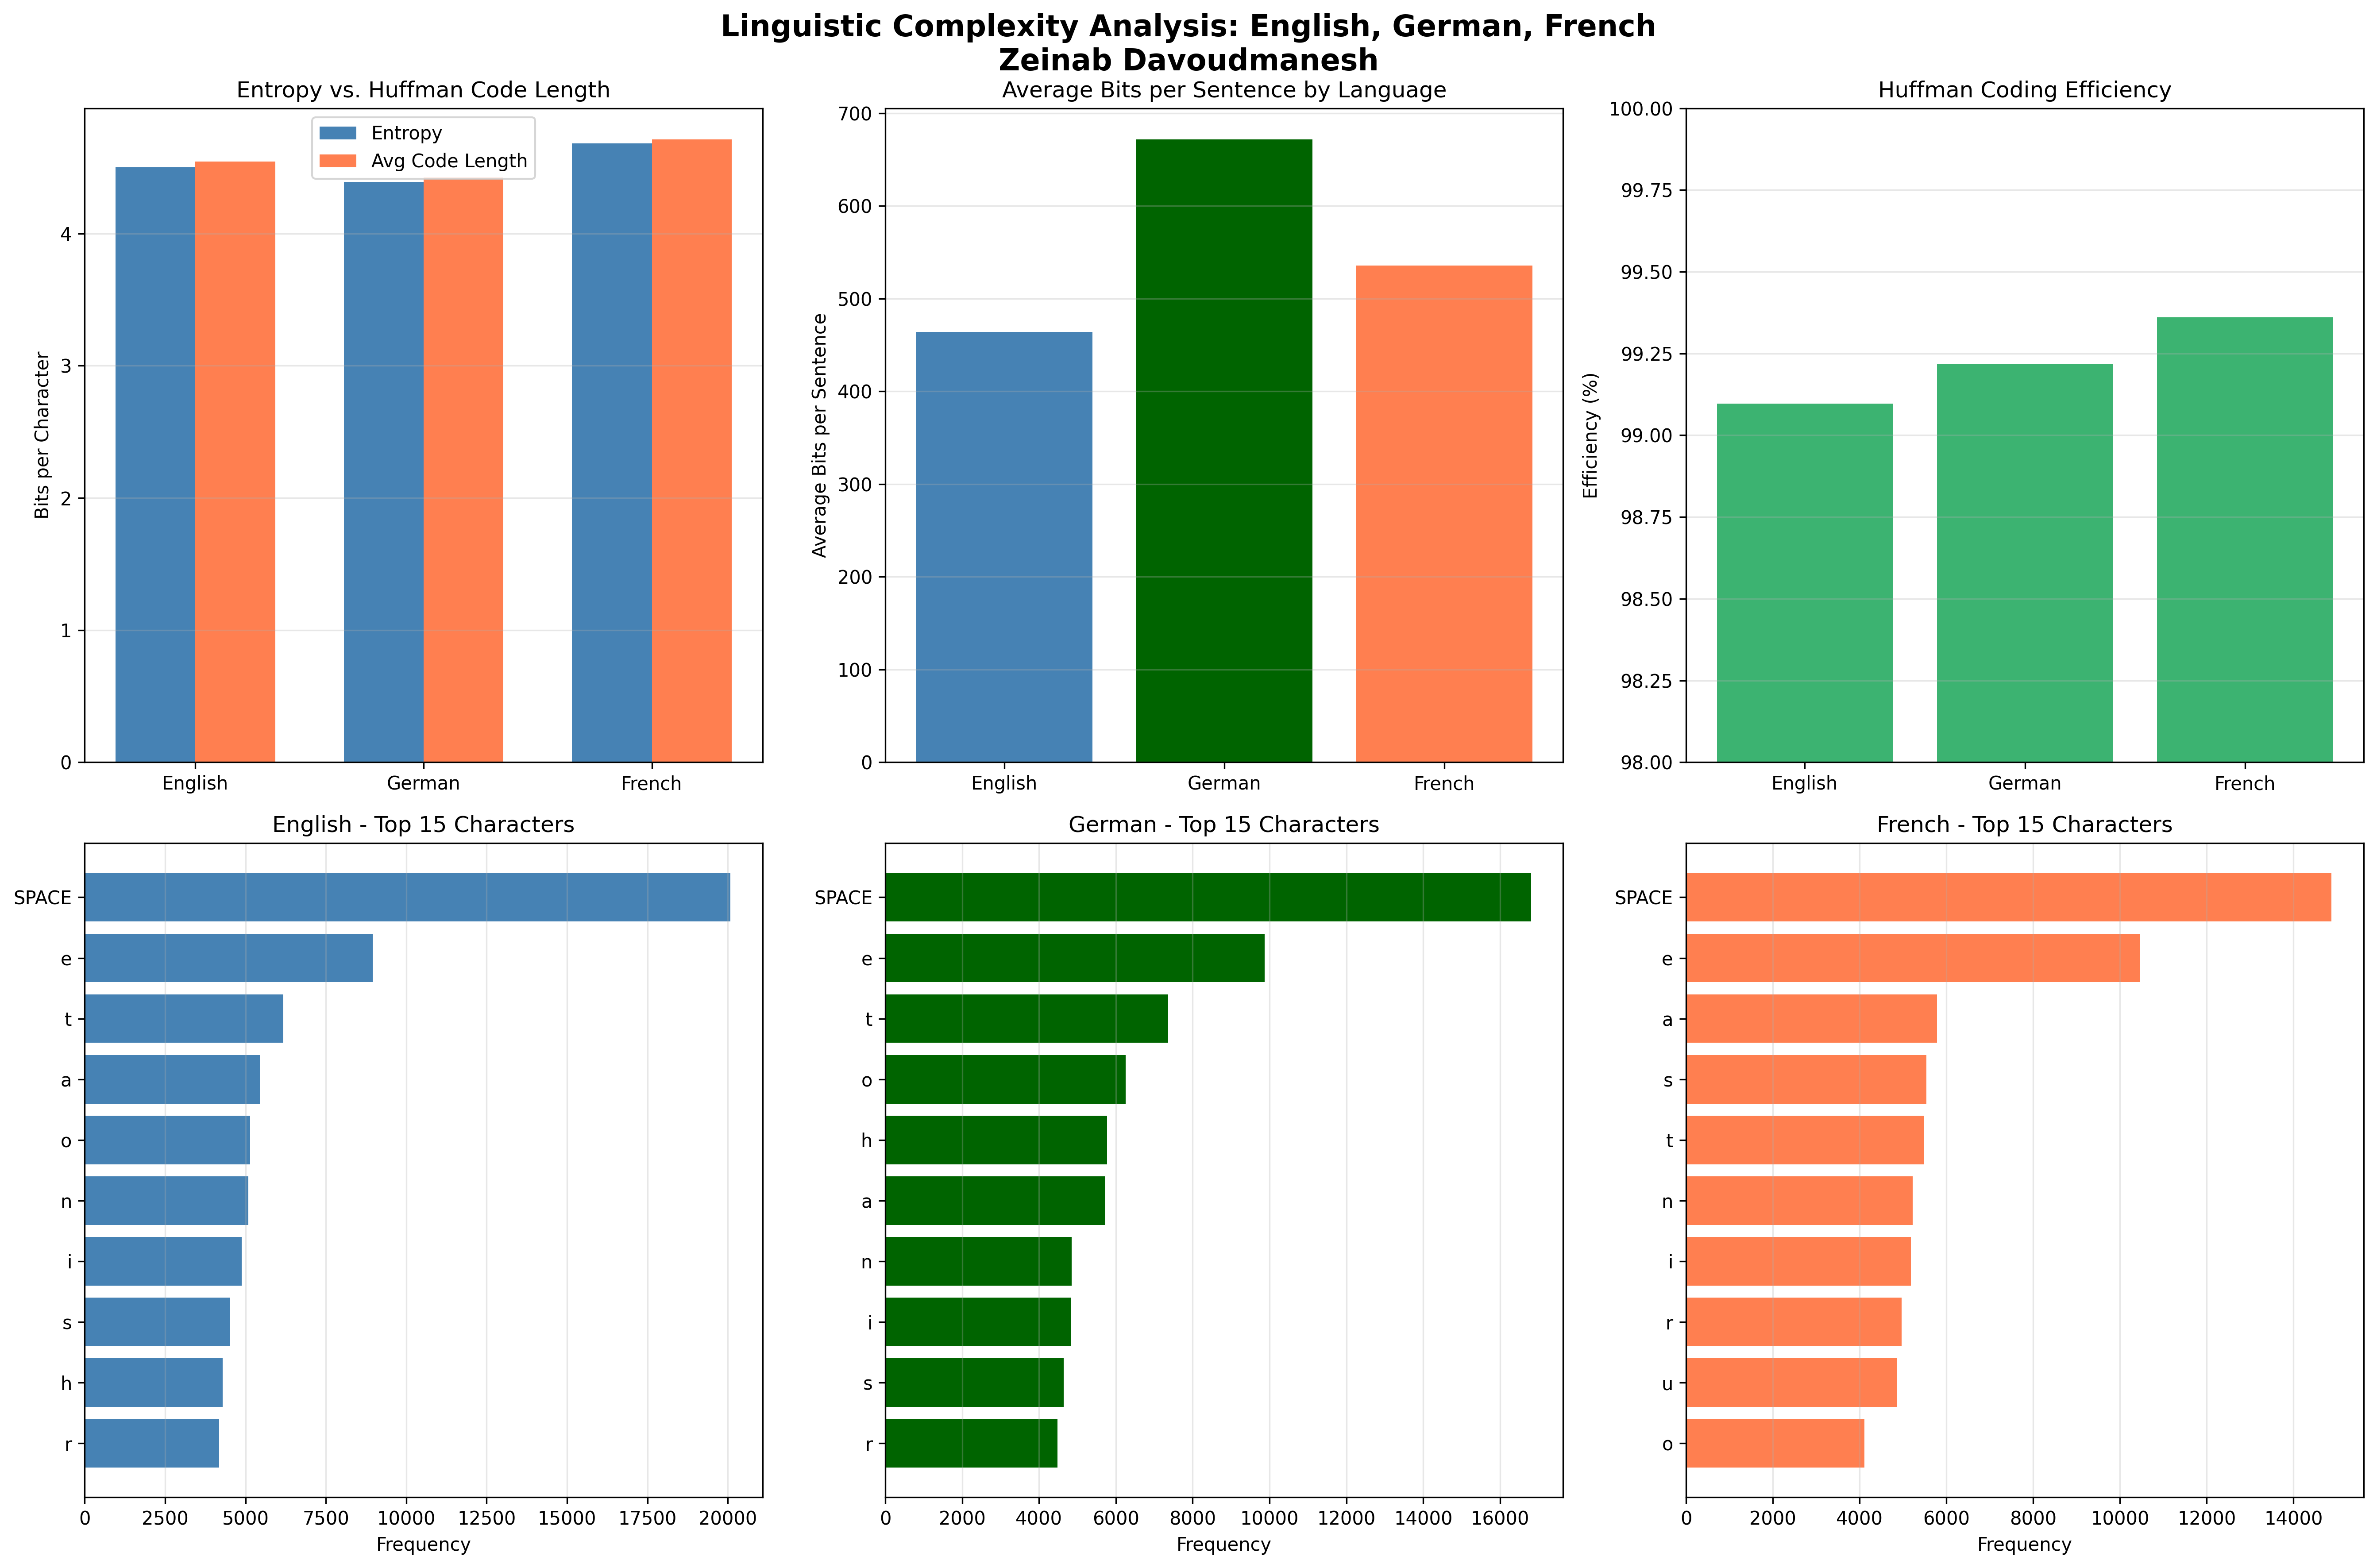
\includegraphics[width=\textwidth]{language_complexity_comparison.png}
\caption{Comprehensive analysis of linguistic complexity across English, German, and French. Top row: (left) entropy vs. code length comparison, (center) average bits per sentence, (right) Huffman coding efficiency. Bottom row: character frequency distributions for each language.}
\label{fig:comparison}
\end{figure}

The visualizations reveal:
\begin{enumerate}
    \item \textbf{Entropy vs. Code Length:} All languages show near-perfect alignment, confirming Huffman optimality
    \item \textbf{Bits per Sentence:} German dominates, followed by French, then English
    \item \textbf{Efficiency:} All three languages achieve 99-100\% efficiency
    \item \textbf{Character Distributions:} Each language shows distinct frequency patterns, with space and 'e' consistently among the most frequent
\end{enumerate}

\section{Discussion}

\subsection{Huffman Coding Efficiency}
The results demonstrate that Huffman coding is highly efficient for natural language text:
\begin{itemize}
    \item English: 99.10\% efficiency
    \item German: 99.22\% efficiency
    \item French: 99.36\% efficiency
\end{itemize}

The small difference between theoretical entropy and actual code length (0.03-0.04 bits) confirms that Huffman coding achieves near-optimal compression for all three languages.

\subsection{Linguistic Complexity}
\textbf{Character-Level Complexity:}

French's higher entropy (4.68 bits/char) reflects its richer alphabet with accented characters (é, è, ê, à, ù, etc.). This greater character diversity requires more information per character to specify which character appears.

German and English have similar entropies (4.39 and 4.50 bits/char), though German's slightly lower value suggests more predictable character patterns, possibly due to more regular orthographic rules and compound word structures.

\textbf{Sentence-Level Complexity:}

The difference in average bits per sentence reveals distinct literary styles:
\begin{itemize}
    \item \textbf{German (672 bits/sentence):} Kafka's philosophical and introspective style in \textit{Die Verwandlung} features complex, layered sentences that explore psychological depth
    \item \textbf{French (536 bits/sentence):} Dumas' adventure narrative uses moderate-length sentences with dramatic flair
    \item \textbf{English (464 bits/sentence):} Austen's dialogue-heavy prose employs shorter, more concise sentences
\end{itemize}

These differences reflect both linguistic structure and authorial style rather than inherent language complexity.

\subsection{Information Theory Implications}
This analysis demonstrates practical applications of Shannon's information theory:
\begin{enumerate}
    \item Entropy quantifies the unpredictability inherent in language
    \item Huffman coding provides a concrete realization of optimal compression
    \item The near-perfect efficiency validates information theory's theoretical predictions
    \item Language exhibits redundancy (entropy $<$ theoretical maximum), enabling compression
\end{enumerate}

\section{Conclusion}
This study successfully analyzed linguistic complexity across English, German, and French using information entropy and Huffman coding. Key findings include:
\begin{enumerate}
    \item French exhibits the highest character-level entropy (4.68 bits/char)
    \item German sentences encode to the most bits on average (672 bits/sentence)
    \item Huffman coding achieves 99\%+ efficiency for all three languages
    \item Character frequency patterns and sentence structures vary significantly across languages
\end{enumerate}

The analysis confirms that information theory provides powerful tools for quantifying linguistic complexity, with practical applications in data compression, natural language processing, and computational linguistics.

\section{Appendix: Python Implementation}

\subsection{Complete Source Code}

\begin{lstlisting}
import heapq
from collections import Counter, defaultdict
import math
import matplotlib.pyplot as plt
import seaborn as sns
import pandas as pd
import numpy as np
import requests

class HuffmanNode:
    def __init__(self, char, freq):
        self.char = char
        self.freq = freq
        self.left = None
        self.right = None
    
    def __lt__(self, other):
        return self.freq < other.freq

class HuffmanCoding:
    def __init__(self, text):
        self.text = text
        self.freq_dict = Counter(text)
        self.huffman_codes = {}
        self.root = None
    
    def build_huffman_tree(self):
        """Build the Huffman tree from character frequencies"""
        heap = [HuffmanNode(char, freq) 
                for char, freq in self.freq_dict.items()]
        heapq.heapify(heap)
        
        while len(heap) > 1:
            left = heapq.heappop(heap)
            right = heapq.heappop(heap)
            
            merged = HuffmanNode(None, left.freq + right.freq)
            merged.left = left
            merged.right = right
            
            heapq.heappush(heap, merged)
        
        self.root = heap[0]
    
    def generate_codes(self, node=None, code=""):
        """Generate Huffman codes for each character"""
        if node is None:
            node = self.root
        
        if node.char is not None:
            self.huffman_codes[node.char] = code if code else "0"
            return
        
        if node.left:
            self.generate_codes(node.left, code + "0")
        if node.right:
            self.generate_codes(node.right, code + "1")
    
    def encode_text(self, text):
        """Encode text using generated Huffman codes"""
        return ''.join(self.huffman_codes[char] for char in text)
    
    def get_average_code_length(self):
        """Calculate average code word length"""
        total_chars = len(self.text)
        total_bits = sum(len(self.huffman_codes[char]) * count 
                        for char, count in self.freq_dict.items())
        return total_bits / total_chars

def calculate_entropy(text):
    """Calculate Shannon entropy of the text"""
    freq_dict = Counter(text)
    total_chars = len(text)
    entropy = 0
    
    for count in freq_dict.values():
        probability = count / total_chars
        entropy -= probability * math.log2(probability)
    
    return entropy

def analyze_language(language_name, text_sample):
    """Complete analysis for one language"""
    # Calculate entropy
    entropy = calculate_entropy(text_sample)
    
    # Build Huffman code
    huffman = HuffmanCoding(text_sample)
    huffman.build_huffman_tree()
    huffman.generate_codes()
    
    avg_code_length = huffman.get_average_code_length()
    
    # Encode sentences
    sentences = split_sentences(text_sample)
    sentence_bits = [len(huffman.encode_text(s)) 
                     for s in sentences if s]
    
    return {
        'entropy': entropy,
        'avg_code_length': avg_code_length,
        'avg_bits_per_sentence': np.mean(sentence_bits)
    }
\end{lstlisting}

\end{document}
